% Options for packages loaded elsewhere
\PassOptionsToPackage{unicode}{hyperref}
\PassOptionsToPackage{hyphens}{url}
%
\documentclass[
]{ctexart}
\usepackage{amsmath,amssymb}
\usepackage{lmodern}
\usepackage{iftex}
\ifPDFTeX
  \usepackage[T1]{fontenc}
  \usepackage[utf8]{inputenc}
  \usepackage{textcomp} % provide euro and other symbols
\else % if luatex or xetex
  \usepackage{unicode-math}
  \defaultfontfeatures{Scale=MatchLowercase}
  \defaultfontfeatures[\rmfamily]{Ligatures=TeX,Scale=1}
\fi
% Use upquote if available, for straight quotes in verbatim environments
\IfFileExists{upquote.sty}{\usepackage{upquote}}{}
\IfFileExists{microtype.sty}{% use microtype if available
  \usepackage[]{microtype}
  \UseMicrotypeSet[protrusion]{basicmath} % disable protrusion for tt fonts
}{}
\makeatletter
\@ifundefined{KOMAClassName}{% if non-KOMA class
  \IfFileExists{parskip.sty}{%
    \usepackage{parskip}
  }{% else
    \setlength{\parindent}{0pt}
    \setlength{\parskip}{6pt plus 2pt minus 1pt}}
}{% if KOMA class
  \KOMAoptions{parskip=half}}
\makeatother
\usepackage{xcolor}
\IfFileExists{xurl.sty}{\usepackage{xurl}}{} % add URL line breaks if available
\IfFileExists{bookmark.sty}{\usepackage{bookmark}}{\usepackage{hyperref}}
\hypersetup{
  pdftitle={一种通过最优子集法结合数据驱动的自适应权重处理小样本超高维类不平衡问题的分类方法},
  pdfauthor={这是测试投稿文件,盗版必究},
  pdfkeywords={小样本, 高维数据, 变量选择, 分类问题},
  hidelinks,
  pdfcreator={LaTeX via pandoc}}
\urlstyle{same} % disable monospaced font for URLs
\usepackage{listings}
\newcommand{\passthrough}[1]{#1}
\lstset{defaultdialect=[5.3]Lua}
\lstset{defaultdialect=[x86masm]Assembler}
\usepackage{longtable,booktabs,array}
\usepackage{calc} % for calculating minipage widths
% Correct order of tables after \paragraph or \subparagraph
\usepackage{etoolbox}
\makeatletter
\patchcmd\longtable{\par}{\if@noskipsec\mbox{}\fi\par}{}{}
\makeatother
% Allow footnotes in longtable head/foot
\IfFileExists{footnotehyper.sty}{\usepackage{footnotehyper}}{\usepackage{footnote}}
\makesavenoteenv{longtable}
\usepackage{graphicx}
\makeatletter
\def\maxwidth{\ifdim\Gin@nat@width>\linewidth\linewidth\else\Gin@nat@width\fi}
\def\maxheight{\ifdim\Gin@nat@height>\textheight\textheight\else\Gin@nat@height\fi}
\makeatother
% Scale images if necessary, so that they will not overflow the page
% margins by default, and it is still possible to overwrite the defaults
% using explicit options in \includegraphics[width, height, ...]{}
\setkeys{Gin}{width=\maxwidth,height=\maxheight,keepaspectratio}
% Set default figure placement to htbp
\makeatletter
\def\fps@figure{htbp}
\makeatother
\setlength{\emergencystretch}{3em} % prevent overfull lines
\providecommand{\tightlist}{%
  \setlength{\itemsep}{0pt}\setlength{\parskip}{0pt}}
\setcounter{secnumdepth}{5}
\lstset{
  breaklines=true,
  basicstyle=\ttfamily
}
\usepackage[ruled]{algorithm2e}
\usepackage{graphicx} %use graph format
\usepackage{epstopdf}
\usepackage{booktabs}
\usepackage{multirow}
\usepackage{xcolor}
\usepackage{listings}
\ifLuaTeX
  \usepackage{selnolig}  % disable illegal ligatures
\fi
\newlength{\cslhangindent}
\setlength{\cslhangindent}{1.5em}
\newlength{\csllabelwidth}
\setlength{\csllabelwidth}{3em}
\newenvironment{CSLReferences}[2] % #1 hanging-ident, #2 entry spacing
 {% don't indent paragraphs
  \setlength{\parindent}{0pt}
  % turn on hanging indent if param 1 is 1
  \ifodd #1 \everypar{\setlength{\hangindent}{\cslhangindent}}\ignorespaces\fi
  % set entry spacing
  \ifnum #2 > 0
  \setlength{\parskip}{#2\baselineskip}
  \fi
 }%
 {}
\usepackage{calc}
\newcommand{\CSLBlock}[1]{#1\hfill\break}
\newcommand{\CSLLeftMargin}[1]{\parbox[t]{\csllabelwidth}{#1}}
\newcommand{\CSLRightInline}[1]{\parbox[t]{\linewidth - \csllabelwidth}{#1}\break}
\newcommand{\CSLIndent}[1]{\hspace{\cslhangindent}#1}

\title{一种通过最优子集法结合数据驱动的自适应权重处理小样本超高维类不平衡问题的分类方法}
\author{这是测试投稿文件,盗版必究}
\date{}

\begin{document}
\maketitle

{
\setcounter{tocdepth}{2}
\tableofcontents
}
\parindent=19pt

\hypertarget{ux6458ux8981}{%
\section{摘要}\label{ux6458ux8981}}

随着科学技术的不断发展,计算机性能的不断提升,现如今的数据呈现指数级增长。如何很好地处理这些海量的数据,以及通过数据处理方法和统计方法,从这些海量的数据之中获取有用的信息,已经成为了现在统计学家们关心的问题。在海量数据的情况下,常常会出现变量数远大于样本数的情况\(p >> n\),这里\(p\)为变量个数,也就是维数,\(n\)为样本数。这是十分棘手的,因为在\(p >> n\)的情况下,很多传统统计中的性质就失去了意义,所建立的统计模型也无法很好的解释事实现象。因此,需要对数据进行变量选择,这里的变量选择是统计中的Variale
selection,随着深度学习地不断发展,现在变量选择更多地情况下被成为特征筛选即Feature
selection。。但从个人角度认为,这两者实际上是一样的,都是从海量的特征之中通过处理方法找到真正起到影响作用的变量或者叫特征。随着变量选择方法的不断提升和改进,我们面对超高维数据的时候也可以进行处理,并且还可以获得一些比较好的性质,如\passthrough{\lstinline!oracle!}性质等。为此,本文尝试使用统计学界的变量选择方法与机器学习方法结合来处理超高维情况下的一些问题。本篇文章结构如下,第二章对前人的方法进行总结叙述,第三章介绍了最优子集方法,第四章通过实际数据进行方法的检验,最终进行了总结和讨论。

\hypertarget{ux6587ux732eux7efcux8ff0}{%
\section{文献综述}\label{ux6587ux732eux7efcux8ff0}}

关于变量选择这一问题,从统计学界的角度来看,比较传统的有逐步回归法,最优子集法等,这些方法可以处理比如多重共线性等问题,但是在\(p\)很大的时候就不是那么有效了,为了处理这一棘手的问题Tibshirani\textsuperscript{{[}1{]}}在1996年提出了\passthrough{\lstinline!lasso!}方法,在回归中加入\(L_1\)惩罚项,巧妙地实现了变量选择。这一方法开拓了变量选择这一方向,在以后的很长一段时间中,许多学者依然是从加入惩罚项这一角度入手,来解决变量选择问题。\passthrough{\lstinline!lasso!}方法从一定程度上解决了高维情况下变量选择的问题,但是由于\(L_1\)范数自身的特性,导致其估计出来的参数无法避免有偏性。为此Fan和Li\textsuperscript{{[}2{]}}在2001年提出SCAD方法,并且提出\passthrough{\lstinline!oracle!}性质。假设\(\mathcal{A}=\left\{j: \beta_{i}^{*} \neq 0\right\}\)并假设\(|\mathcal{A}|=p_{0}<p\),因此假设真实的模型是取决于自变量的子集,即这里\(\mathcal{A}\)为真实的模型。这里将\(\hat{\boldsymbol{\beta}}(\delta)\)记为通过方法\(\delta\)拟合出来的参数估计值。\(\hat{\boldsymbol{\beta}}(\delta)\)的\passthrough{\lstinline!oracle!}性质即为:

\begin{itemize}
\tightlist
\item
  能够找到真实的子集,\(\lim _{n} P\left(\mathcal{A}_{n}^{*}=\mathcal{A}\right)=1\)
\item
  有渐进正态性质,\(\sqrt{n}\left(\boldsymbol{\beta}(\delta)_{\mathcal{A}}-\boldsymbol{\beta}_{\mathcal{A}}^{*}\right) \rightarrow_{d}\mathrm{N}\left(\mathbf{0}, \boldsymbol{\Sigma}^{*}\right)\)。依分布收敛与真实的参数收敛到正态分布。这里\(\boldsymbol{\Sigma}^{*}\)是真实子模型的协方差矩阵。
\end{itemize}

在Fan提出\passthrough{\lstinline!oracle!}性质之后,传统的\passthrough{\lstinline!lasso!}方法并不能满足\passthrough{\lstinline!oracle!}性质,Fan提出的SCAD方法能够满足\passthrough{\lstinline!oracle!}性质,从而进一步提升了变量选择方法的性能。在以后的很长一段时间,一个变量选择方法是否能够满足\passthrough{\lstinline!oracle!}性质成为了判别其好坏的主要评判标准。Zou\textsuperscript{{[}3{]}}等人在2005年提出弹性网模型,创新地将\passthrough{\lstinline!lasso!}和\passthrough{\lstinline!ridge!}方法的\(L_1\)和\(L_2\)范数结合到一起,弹性网模型能够较好的解决数据中存在较强相关的两个变量的情况,Zou通过数学方法巧妙地证明了弹性网模型能够很好的解决这一问题,并在处理医学基因数据中得到了很好的结果。
Efron等人\textsuperscript{{[}4{]}}在2005年提出了\passthrough{\lstinline!least angel regression!}方法,该算法提升了\passthrough{\lstinline!lasso!}方法,并且可以快速计算出\passthrough{\lstinline!lasso!}方法的参数估计值,并且解释了\passthrough{\lstinline!lasso!}和向前回归法的联系。Meinshausen\textsuperscript{{[}5{]}}等人在2006年提出了图\passthrough{\lstinline!lasso!}方法,进一步提升了\passthrough{\lstinline!lasso!}方法的使用范围。接着Zou\textsuperscript{{[}6{]}}等人提出\passthrough{\lstinline!adaptive lasso!}方法,该方法通过创新地将惩罚项之前加入根据样本计算的系数\(\omega\),这里\(\omega\)可以是根据样本计算出的普通最小二乘的系数,即\(\underset{\boldsymbol{\beta}}{\arg \min }\left\|\mathbf{y}-\sum_{j=1}^{p} \mathbf{x}_{j} \beta_{j}\right\|^{2}+\lambda \sum_{j=1}^{p} w_{j}\left|\beta_{j}\right|\),通过进行加权的方法,使传统的\passthrough{\lstinline!lasso!}方法有了适应性,并且Zou证明了\passthrough{\lstinline!adaptive lasso!}方法具有\passthrough{\lstinline!oracle!}性质,从而极大的提升了\passthrough{\lstinline!lasso!}方法的性能。Candes\textsuperscript{{[}7{]}}等人在2007年提出\passthrough{\lstinline!dantzig selector!}方法,该方法即是求解\(\min \|\hat{\beta}\|_{1} \quad\)
s.t.
\(\quad\left\|\boldsymbol{X}^{\prime} r\right\|_{\infty} \leq \lambda_{p} \cdot \sigma\),该方法限制目标函数的梯度在\(\lambda\)内,该方法与\passthrough{\lstinline!lasso!}方法差别非常小,可以看作是受\passthrough{\lstinline!lasso!}的kkt条件启发而给出的优化范式。

至此为止,本文讨论了从Tibshirani开始开创的使用惩罚项的变量选择方法,从1996年开始,这一方法基本占据了变量选择的主流,并且在实际应用当中取得了很好的效果。并且变量选择的方法也与兴起的机器学习产生了交叉,通过使用统计中的变量选择方法来处理机器学习中的问题也成为了一种方式。本文对传统的变量选择方法总结如下,只列出部分方法。

\begin{table}[htb]
\centering
\caption{表一 传统变量选择方法比较}
\begin{tabular}{ccccl}
\cline{1-4}
\multicolumn{4}{c}{传统变量选择比较} &  \\
方法      & 无偏性  & 连续性  & 稀疏性  &  \\ \cline{1-4}
LASSO   & 无    & 无    & 有    &  \\
SCAD    & 有    & 有    & 有    &  \\
Ridge   & 有    & 有    & 无    &  \\
硬门限     & 有    & 无    & 有    &  \\ \cline{1-4}
\end{tabular}
\end{table}

在2008年,Fan\textsuperscript{{[}8{]}}提出了Sure independence
screening方法(以下简称SIS方法),该方法将变量选择从传统的惩罚项的改进方面提供了一个新的视野,其实SIS方法就是对每个变量计算其与因变量\(y\)的皮尔逊相关系数\(r\),然后根据相关系数的大小排序进行变量的选择。这种看起来十分简单粗暴的办法,在处理超高维数据时也会有不错的效果。Fan在其中提出了SIS性质如下,将\(\mathcal{M}_{*}\)记为真实的模型,\(\mathcal{M}_{\gamma}\)记为最终的模型。\[P\left(\mathcal{M}_{*} \subset \mathcal{M}_{\gamma}\right) \rightarrow 1 \quad \text { as } n \rightarrow \infty\]

即在样本量\(n\)趋近于无穷的时候,真实模型属于最终模型的概率趋近于1。这种性质能够很好地保证最终筛选出来的模型与真实的模型有一致性。在Fan提出该方法之后其本人在2010年\textsuperscript{{[}9{]}}提出了对SIS方法的改进,将SIS方法拓展到广义线性模型之中,并改变了SIS方法中的参数估计方法,从之前的相关系数拓展到极大边际似然统计量,进一步提升了SIS方法的引用范围。之后Li\textsuperscript{{[}10{]}}等人在2012年提出了基于距离关联的SIS方法(简称为DC-SIS),将Fan之前的单纯使用皮尔逊相关系数的方法拓展到了更大的范围,该方法放宽了SIS方法对自变量和因变量的限制条件,但是DC-SIS方法失去了SIS性质,也有一定的局限性。

通过对前人方法的总结,传统的方法在处理变量选择问题的时候基本都不可避免的会受到模型假定条件的限制或者统计性质的局限,其实在统计方法内,对变量选择最好的方法是最优子集法,但是其高昂的计算成本让其在之前成为了一种相对不可行的方法,但是Zhu\textsuperscript{{[}11{]}}在2020年提出了一种计算最优子集的算法,将其从不可能变为了可能。

\hypertarget{ux65b9ux6cd5ux7b80ux4ecb}{%
\section{方法简介}\label{ux65b9ux6cd5ux7b80ux4ecb}}

\hypertarget{ux6700ux4f18ux5b50ux96c6ux6cd5ux7b80ux4ecb}{%
\subsection{最优子集法简介}\label{ux6700ux4f18ux5b50ux96c6ux6cd5ux7b80ux4ecb}}

最优子集法即\passthrough{\lstinline!best subset selection!},最早可见Hocking\textsuperscript{{[}12{]}}等人1967年的文章,其思想十分简单。从零号模型(null
model)\(M_0\)开始,这个模型只有截距项而没有任何自变量。然后用不同的特征组合进行拟合,从特征中分别挑选出一个最好的模型(RSS最小或\(R^2\)最大),也就是包含1个特征的模型\(M_1\),包含2个特征的模型\(M_2\),直至包含p个特征的模型\(M_p\)。然后从这总共p+1个模型中选出其中最好的模型(根据交叉验证误差,\(C_p\),BIC或adjusted
\(R^2\))(注:为什么不能用RSS或\(R^2\)来衡量?因为增加任何特征,模型的训练RSS只会变小,\(R^2\)只会增大)。这个最好模型所配置的特征就是筛选出的特征。最优子集法在理想的条件下可以筛选出最好的特征集合出来,但是其高昂的计算成本是阻碍其应用的主要问题。Zhu\textsuperscript{{[}11{]}}等人在2021年提出了一种最优子集法的多项式算法,证明了在一定条件下,该算法具有以下三个优良性质:

\begin{itemize}
\tightlist
\item
  计算复杂度是多项式的
\item
  选择出来的子集能够覆盖真实的集合
\item
  该算法的解是全局最优的
\end{itemize}

作者将该方法称为\passthrough{\lstinline!Adaptive Best-Subset Selection!}以下简称\passthrough{\lstinline!BeSS!},在作者提出的SIC(special
information
criterion)准则下,该方法的模型选择连续性得到了证明。SIC准则如下:
\[\operatorname{SIC}(\mathcal{A})=n \log \mathcal{L}_{\mathcal{A}}+|\mathcal{A}| \log (p) \log \log n\]
其中\(\mathcal{A}\)为筛选出来的特征的集合。

\hypertarget{ux526aux63a5ux65b9ux6cd5ux7b80ux4ecb}{%
\subsection{剪接方法简介}\label{ux526aux63a5ux65b9ux6cd5ux7b80ux4ecb}}

首先定义一些变量名称,\(\boldsymbol{\beta}=\left(\beta_{1}, \ldots, \beta_{p}\right)^{\top} \in \mathbb{R}^{p}\),将\(\ell_{q}\)定义为:\(\|\boldsymbol{\beta}\|_{q}=\left(\sum_{j=1}^{p}\left|\beta_{j}\right|^{q}\right)^{1 / q},q \in[1, \infty)\)。\(\mathcal{S}=\{1, \ldots, p\}\),对任何\(\mathcal{A} \subseteq \mathcal{S}\),记\(\mathcal{A}^{c}=\mathcal{S} \backslash \mathcal{A}\)作为\(\mathcal{A}\)的补集,\(|\mathcal{A}|\)作为他的基。将\(\beta\)的子集定义为\(\operatorname{supp}(\boldsymbol{\beta})=\left\{j: \beta_{j} \neq 0\right\}\)。对一个指标集\(\mathcal{A} \subseteq\{1, \ldots, p\}\),\(\boldsymbol{\beta}_{\mathcal{A}}=\left(\beta_{j}, j \in \mathcal{A}\right) \in \mathbb{R}^{|\mathcal{A}|}\)。对一个矩阵\(\boldsymbol{X} \in \mathbb{R}^{n \times p}\)定义\(\boldsymbol{X}_{\mathcal{A}} =(X_{j},j \in \mathcal{A}) \in \mathbb{R}^{n \times|\mathcal{A}|}\)。对任何一个向量\(t\)和任何一个集合\(\mathcal{A}\),\(t^{\mathcal{A}}\)是一个第\(j\)个元素\(\left(\boldsymbol{t}^{\mathcal{A}}\right)_{j}\)如果\(j \in \mathcal{A}\)就等于\(t_{j}\),否则为0。

在文章中,作者最重要的贡献是提出了剪接方法,即\passthrough{\lstinline!splicing method!},通过使用该种方法,显著的提升了最优子集算法的性能,使其在当前的环境下变的可行。
考虑\(\ell_{0}\)限制最小化问题:\[
\min _{\boldsymbol{\beta}} \mathcal{L}_{n}(\boldsymbol{\beta}), \quad \text { s. } t\|\boldsymbol{\beta}\|_{0} \leq \boldsymbol{s}
\]
其中:\(\mathcal{L}_{n}(\boldsymbol{\beta})=\frac{1}{2 n}\|\boldsymbol{y}-\boldsymbol{X} \boldsymbol{\beta}\|_{2}^{2}\)。在不考虑全局损失的情况下,我们考虑\(\|\boldsymbol{\beta}\|_{0}=\boldsymbol{s}\)。给定一个初始集合\(\mathcal{A} \subset \mathcal{S}=\{1,2, \ldots, p\}\),且\(|\mathcal{A}|=s\),记\(\mathcal{I}=\mathcal{A}^{c}\)并且计算\[
\hat{\boldsymbol{\beta}}=\arg \min _{\boldsymbol{\beta}_{\mathcal{I}}=0} \mathcal{L}_{n}(\boldsymbol{\beta})
\]
将\(\mathcal{A}\)和\(\mathcal{I}\)定义为激活集合和非激活集合,这里的激活就是在真实集合中的意思。在给定了\(\mathcal{A}\)和\(\hat{\beta}\)之后,可以定义两种损失如下:

\begin{itemize}
\item
  后退损失\[
  \xi_{j}=\mathcal{L}_{n}\left(\hat{\boldsymbol{\beta}}^{\mathcal{A} \backslash\{j\}}\right)-\mathcal{L}_{n}\left(\hat{\boldsymbol{\beta}}^{\mathcal{A}}\right)=\frac{\boldsymbol{X}_{j}^{\top} \boldsymbol{X}_{j}}{2 n}\left(\hat{\beta}_{j}\right)^{2}
  \]
\item
  前进损失:\[
  \zeta_{j}=\mathcal{L}_{n}\left(\hat{\boldsymbol{\beta}}^{\mathcal{A}}\right)-\mathcal{L}_{n}\left(\hat{\boldsymbol{\beta}}^{\mathcal{A}}+\hat{\boldsymbol{t}}^{\{j\}}\right)=\frac{\boldsymbol{X}_{j}^{\top} \boldsymbol{X}_{j}}{2 n}\left(\frac{\hat{d}_{j}}{\boldsymbol{X}_{j}^{\top} \boldsymbol{X}_{j} / n}\right)^{2}
  \]
  其中:\(\hat{t}=\arg \min _{t} \mathcal{L}_{n}\left(\hat{\boldsymbol{\beta}}^{\mathcal{A}}+\boldsymbol{t}^{\{j\}}\right), \hat{d}_{j}=\boldsymbol{X}_{j}^{\top}(\boldsymbol{y}-\boldsymbol{X} \hat{\boldsymbol{\beta}}) / n\)
\end{itemize}

直观的而言,对\(j \in \mathcal{A}\)一个大的\(\xi_{j}\)说明这个变量是潜在重要的。但是由于子集大小不同,这两个损失是无法比较的。然而如果将\(\mathcal{A}\)中的一些不是那么相关的变量和\(\mathcal{I}\)中一些重要的变量交换,这也许能够获得比较好的结果,这就是剪接法的思想所在。
特别的,对任何给定的\(k <= s\)定义如下: \[
\mathcal{A}_{k}=\left\{j \in \mathcal{A}: \sum_{i \in \mathcal{A}} \mathrm{I}\left(\xi_{j} \geq \xi_{i}\right) \leq k\right\}
\] \[
\mathcal{I}_{k}=\left\{j \in \mathcal{I}: \sum_{i \in \mathcal{I}} \mathrm{I}\left(\zeta_{j} \leq \zeta_{i}\right) \leq k\right\}
\]
通过交换\(\mathcal{A}_{k}\)和\(\mathcal{I}_{k}\),从而实现对\(\mathcal{A}\)和\(\mathcal{I}\)的切片,得到了新的集合:
\[
\tilde{\mathcal{A}}=\left(\mathcal{A} \backslash \mathcal{A}_{k}\right) \cup \mathcal{I}_{k}
\]
记\(\tilde{\mathcal{I}}=\tilde{\mathcal{A}}^{c}, \tilde{\boldsymbol{\beta}}=\arg \min _{\boldsymbol{\beta}_{\tilde{\mathcal{I}}}=0} \mathcal{L}_{n}(\boldsymbol{\beta})\),并且\(\tau_{s}>0\)为阈值。如果\(\tau_{s} < \mathcal{L}_{n}(\hat{\boldsymbol{\beta}})-\mathcal{L}_{n}(\tilde{\boldsymbol{\beta}})\)
则说明\(\tilde{\mathcal{A}}\)是优于\(\mathcal{A}\)。通过这样的方法则可以更新集合\(\mathcal{A}\)指导损失函数不能够通过剪接方法来进行提升。还有的问题就是设定初始集。通常来说我们选定第一批\(s\)个特征,这些特征是与\(y\)关联程度最大的特征。设\(k_{max}\)为剪接最大尺寸,\(k_{max}<s\),接下来的算法演示了如何计算具体的方法。

\begin{algorithm}[H]
\caption{计算初始集合算法}%算法名字
\KwIn{输入参数$X$,$y$,正整数$k_{max}$和阈值$\tau_{s}$,$\mathcal{A}^{0}=\left\{j: \sum_{i=1}^{p} \mathrm{I}\left(\left|\frac{\boldsymbol{x}_{j}^{\top} \boldsymbol{y}}{\sqrt{\boldsymbol{x}_{j}^{\top} \boldsymbol{x}_{j}}}\right| \leq \mid \frac{\boldsymbol{x}_{i}^{\top} \boldsymbol{y}}{\sqrt{\boldsymbol{x}_{i}^{\top} \boldsymbol{x}_{i}}} \leq \mathrm{s}\right\}, \mathcal{I}^{0}=\left(\mathcal{A}^{0}\right)^{c}\right.$,\;$\left(\boldsymbol{\beta}^{0}, \boldsymbol{d}^{0}\right):$
$\boldsymbol{\beta}_{\mathcal{T}^{0}}^{0}=0$,
$\boldsymbol{d}_{\mathcal{A}^{0}}^{0}=0$,
$\boldsymbol{\beta}_{\mathcal{A}^{0}}^{0}=\left(\boldsymbol{X}_{\mathcal{A}^{0}}^{\top} \boldsymbol{X}_{\mathcal{A}^{0}}\right)^{-1} \boldsymbol{X}_{\mathcal{A}^{0}}^{\top} \boldsymbol{y}_{\boldsymbol{I}}$
$\boldsymbol{d}_{\mathcal{I}^{0}}^{0}=\boldsymbol{X}_{\mathcal{I}^{0}}^{\top}\left(\boldsymbol{y}-\boldsymbol{X} \boldsymbol{\beta}^{0}\right) / n$}%输入参数
\KwOut{$(\hat{\boldsymbol{\beta}}, \hat{\boldsymbol{d}}, \hat{\mathcal{A}}, \hat{\mathcal{I}})=\left(\boldsymbol{\beta}^{m+1}, \boldsymbol{d}^{m+1} \mathcal{A}^{m+1}, \mathcal{I}^{m+1}\right)$}%输出
计算初始集合\; %\;用于换行
\For{$m=0,1,2,3....$}{
  $\left(\boldsymbol{\beta}^{m+1}, \boldsymbol{d}^{m+1},{\mathcal{A}}^{m+1},{\mathcal{I}}^{m+1}\right)=\operatorname{Splicing}\left(\boldsymbol{\beta}^{m}, \boldsymbol{d}^{m}, \mathcal{A}^{m}, \mathcal{I}^{m}, k_{\max }, \tau_{s}\right)$\;
}
\If{$\left(\mathcal{A}^{m+1}, \mathcal{I}^{m+1}\right)=\left(\mathcal{A}^{m}, \mathcal{I}^{m}\right)$}{
    stop\;
  }
\end{algorithm}

\begin{algorithm}[H]
\caption{剪接算法}%算法名字
\KwIn{$\boldsymbol{\beta}, \boldsymbol{d}, \mathcal{A}, \mathcal{I}, k_{\max }$,  $\tau_{s}$,$L_{0}=L=\frac{1}{2 n}\|\boldsymbol{y}-\boldsymbol{X} \boldsymbol{\beta}\|_{2^{\prime}}^{2}$,$\xi_{j}=\frac{x_{j}^{\top} x_{j}}{2 n}\left(\beta_{j}\right)^{2}, \zeta_{j}=\frac{x_{j}^{\top} x_{j}}{2 n}\left(\frac{d_{j}}{x^{\top} x_{i} / n}\right)^{2}, j=1, \ldots, p$}%输入参数
\KwOut{$(\hat{\boldsymbol{\beta}}, \hat{\boldsymbol{d}}, \hat{\mathcal{A}}, \hat{\mathcal{I}})$}%输出
进行剪接算法\; %\;用于换行
\For{$k=0,1,2,3....k_{max}$}{
 $\mathcal{A}_{k}=\left\{j \in \mathcal{A}: \sum_{i \in \mathcal{A}} \mid\left(\xi_{j} \geq \xi_{i}\right) \leq k\right\}$\;
 $\mathcal{I}_{k}=\left\{j \in \mathcal{I}: \sum_{i<\mathcal{T}} \mid\left(\zeta_{j} \leq \zeta_{i}\right) \leq k\right\}$\;
 让$\tilde{\mathcal{A}}_{k}=\left(\mathcal{A} \backslash \mathcal{A}_{k}\right) \cup \mathcal{I}_{k}, \tilde{\mathcal{I}}_{k}=\left(\mathcal{I} \backslash \mathcal{I}_{k}\right) \cup \mathcal{A}_{k}$并求\;
 $\tilde{\boldsymbol{\beta}}_{\tilde{\mathcal{A}}_{k}}=\left(\boldsymbol{x}_{\tilde{\mathcal{A}}_{k}}^{\top} \boldsymbol{x}_{\tilde{\mathcal{A}}_{k}}\right)^{-1} \boldsymbol{X}_{\tilde{\mathcal{A}}_{k}}^{\top} y_{1}, \tilde{\boldsymbol{\beta}}_{\tilde{\mathcal{I}}_{k}}=0$\;
 $\tilde{\boldsymbol{d}}=\boldsymbol{X}^{\top}(\boldsymbol{y}-\boldsymbol{X} \tilde{\boldsymbol{\beta}}) / n, \quad \mathcal{L}_{n}(\tilde{\boldsymbol{\beta}})=\frac{1}{2 n}\|\boldsymbol{y}-\boldsymbol{X} \tilde{\boldsymbol{\beta}}\|_{2}^{2}$\;
}
\If{$L>\mathcal{L}_{n}(\tilde{\boldsymbol{\beta}})$}{
    $(\hat{\boldsymbol{\beta}}, \hat{\boldsymbol{d}}, \hat{\mathcal{A}}, \hat{\mathcal{I}})=\left(\tilde{\boldsymbol{\beta}}, \tilde{\boldsymbol{d}}, \tilde{\mathcal{A}}_{k}, \tilde{\mathcal{I}}_{k}\right)$\;
    $L=\mathcal{L}_{n}(\tilde{\boldsymbol{\beta}}) .$\;
    end for
  }
\If{$L_{0}-L<\tau_{s}$}{$(\hat{\boldsymbol{\beta}}, \hat{\boldsymbol{d}}, \hat{\mathcal{A}}, \hat{\mathcal{I}})=(\boldsymbol{\beta}, \boldsymbol{d}, \mathcal{A}, \mathcal{I})$}
输出结果
\end{algorithm}

通过如上两个算法,Zhu等人巧妙地将最优子集法的计算问题转化为了可以计算的实际应用算法。

\hypertarget{ux7c7bux4e0dux5e73ux8861ux95eeux9898ux52a0ux6743ux65b9ux6cd5}{%
\subsection{类不平衡问题加权方法}\label{ux7c7bux4e0dux5e73ux8861ux95eeux9898ux52a0ux6743ux65b9ux6cd5}}

在进行分类问题时,经常会遇到类不平衡问题,具体表现为某一类的个数明显的超过了另一类,尤其是在处理二分类问题时。对类不平衡问题,常见地处理方法有加权方法和抽样方法。抽样方法有欠采样和过采样,对少的类进行过采样,对多的类进行欠采样,通过这样的方法来使类不平衡的问题得到处理,详见Li\textsuperscript{{[}13{]}},Tang\textsuperscript{{[}14{]}}和Zou\textsuperscript{{[}15{]}}等人
这些前人研究了类不平衡问题在支持向量机中的解决方法,这里我们受到他们思想的启发。

另一种处理类不平衡问题的方法是加权方法,详见Hwang\textsuperscript{{[}16{]}}等人。将正例点个数记为\(N_{pos}\),将负例点个数记为\(N_{neg}\),最常用的权重为如下权重:
\[
w_{i}=\left\{\begin{array}{ll}
1 / N_{\text {pos }} & \text { if } y_{i}=1 \\
1 / N_{\text {neg }} & \text { otherwise }
\end{array}\right.
\]
然而,Hwang设计了一种不同的权重方式,来提升算法的收敛速度,新的权重为:
\[
w_{i}=\left\{\begin{array}{ll}
1 & \text { if } y_{i}=1, \quad N_{p o s} \geq N_{n e g} \\
N_{n e g} / N_{p o s} & \text { if } y_{i}=1, \quad N_{p o s}<N_{n e g} \\
N_{p o s} / N_{n e g} & \text { if } y_{i}=-1, \quad N_{p o s} \geq N_{n e g} \\
1 & \text { if } y_{i}=-1, \quad N_{p o s}<N_{n e g}
\end{array}\right.
\]
该权重不仅能够保留比率,并且能够使收敛速度更快。本文采用该思想,对数据进行加权处理。

\hypertarget{ux6a21ux62dfux5b9eux8bc1}{%
\section{模拟实证}\label{ux6a21ux62dfux5b9eux8bc1}}

本文考虑使用BeSS方法和加权方法来处理超高维且类不平衡条件下的二分类问题,在该条件下,将BeSS方法的回归模型设置为logstic模型,从而得到分类结果。
首先使用较为标准的数据集合进行模拟计算,然后使用真实的数据集来验证我们的方法是否具有可行性。在这里我们将我们的方法命名为\passthrough{\lstinline!WBESS(weighted bess)!}
使用UCI数据库的RNA序列数据,共有800个样本,20000个特征数,每个样本的类别是其所患肿瘤的类型不同,将该数据集合使用不同的方法进行建模,得到二分类结果,从而验证BeSS方法和加权方法对该类问题是否能够有所提升。

\hypertarget{ux6a21ux62dfux8ba1ux7b97}{%
\subsection{模拟计算}\label{ux6a21ux62dfux8ba1ux7b97}}

在这个例子中,本文生成250个正例和350个负例点,正例点的均值为+2,负例点的均值为-2,数据维度为400维。使用自适应加权支持向量机得到的混淆矩阵结果如下。横轴为预测结果,纵轴为原始标签。
总共有三种情况如下所示:

\begin{itemize}
\tightlist
\item
  情况1:正例250个,负例350个,维度为400
\item
  情况2:正例250个,负例500个,维度为400
\item
  情况3:正例250个,负例500个,维度为1000
\end{itemize}

\hypertarget{ux60c5ux51b51}{%
\subsubsection{情况1}\label{ux60c5ux51b51}}

\begin{longtable}[]{@{}lrr@{}}
\caption{使用自适应加权支持向量机分类结果}\tabularnewline
\toprule
& -1 & 1 \\
\midrule
\endfirsthead
\toprule
& -1 & 1 \\
\midrule
\endhead
-1 & 57 & 14 \\
1 & 13 & 36 \\
\bottomrule
\end{longtable}

使用传统支持向量机结果如下表所示。

\begin{longtable}[]{@{}lrr@{}}
\caption{使用传统支持向量机混淆矩阵}\tabularnewline
\toprule
& -1 & 1 \\
\midrule
\endfirsthead
\toprule
& -1 & 1 \\
\midrule
\endhead
-1 & 60 & 45 \\
1 & 3 & 12 \\
\bottomrule
\end{longtable}

使用logstic回归结果如下:

\begin{longtable}[]{@{}lrr@{}}
\caption{使用logstic回归结果}\tabularnewline
\toprule
& -1 & 1 \\
\midrule
\endfirsthead
\toprule
& -1 & 1 \\
\midrule
\endhead
-1 & 47 & 17 \\
1 & 19 & 37 \\
\bottomrule
\end{longtable}

使用BeSS方法结果的混淆矩阵如下:

\begin{longtable}[]{@{}lrr@{}}
\caption{使用BeSS结果}\tabularnewline
\toprule
& -1 & 1 \\
\midrule
\endfirsthead
\toprule
& -1 & 1 \\
\midrule
\endhead
-1 & 61 & 8 \\
1 & 5 & 46 \\
\bottomrule
\end{longtable}

计算各个方法的指数如下表所示:

\begin{longtable}[]{@{}cccccc@{}}
\caption{250个正例和300个负例情况下各种方法参数对比}\tabularnewline
\toprule
method & Sensitivity & Specificity & FPR & FNR & ACC \\
\midrule
\endfirsthead
\toprule
method & Sensitivity & Specificity & FPR & FNR & ACC \\
\midrule
\endhead
awensvm & 73.46 & 80.28 & 18.30 & 18.57 & 77.50 \\
svm & 80.00 & 57.14 & 2.80 & 4.76 & 60.00 \\
BeSS & 90.19 & 88.40 & 7.20 & 7.57 & 89.16 \\
logstic & 66.07 & 73.43 & 29.68 & 28.78 & 70.00 \\
\bottomrule
\end{longtable}

\begin{figure}
\includegraphics{test_files/figure-latex/unnamed-chunk-7-1} \caption{250个正例和300个负例情况下各种方法比较图}\label{fig:unnamed-chunk-7}
\end{figure}

\hypertarget{ux60c5ux51b52}{%
\subsubsection{情况2}\label{ux60c5ux51b52}}

接着本文生成250个正例点和500个负例点来对比各种方法的效果,结果如下表所示。

\begin{longtable}[]{@{}cccccc@{}}
\caption{250个正例和500负例情况下各种方法指标比对}\tabularnewline
\toprule
method & Sensitivity & Specificity & FPR & FNR & ACC \\
\midrule
\endfirsthead
\toprule
method & Sensitivity & Specificity & FPR & FNR & ACC \\
\midrule
\endhead
awensvm & 69.49 & 93.40 & 6.59 & 30.50 & 84.00 \\
svm & 12.50 & 100.00 & 0.00 & 42.60 & 72.00 \\
logstic & 89.58 & 76.47 & 23.52 & 10.41 & 78.28 \\
BeSS & 100.00 & 100.00 & 0.00 & 0.00 & 100.00 \\
\bottomrule
\end{longtable}

可视化结果如下图所示。

\begin{figure}
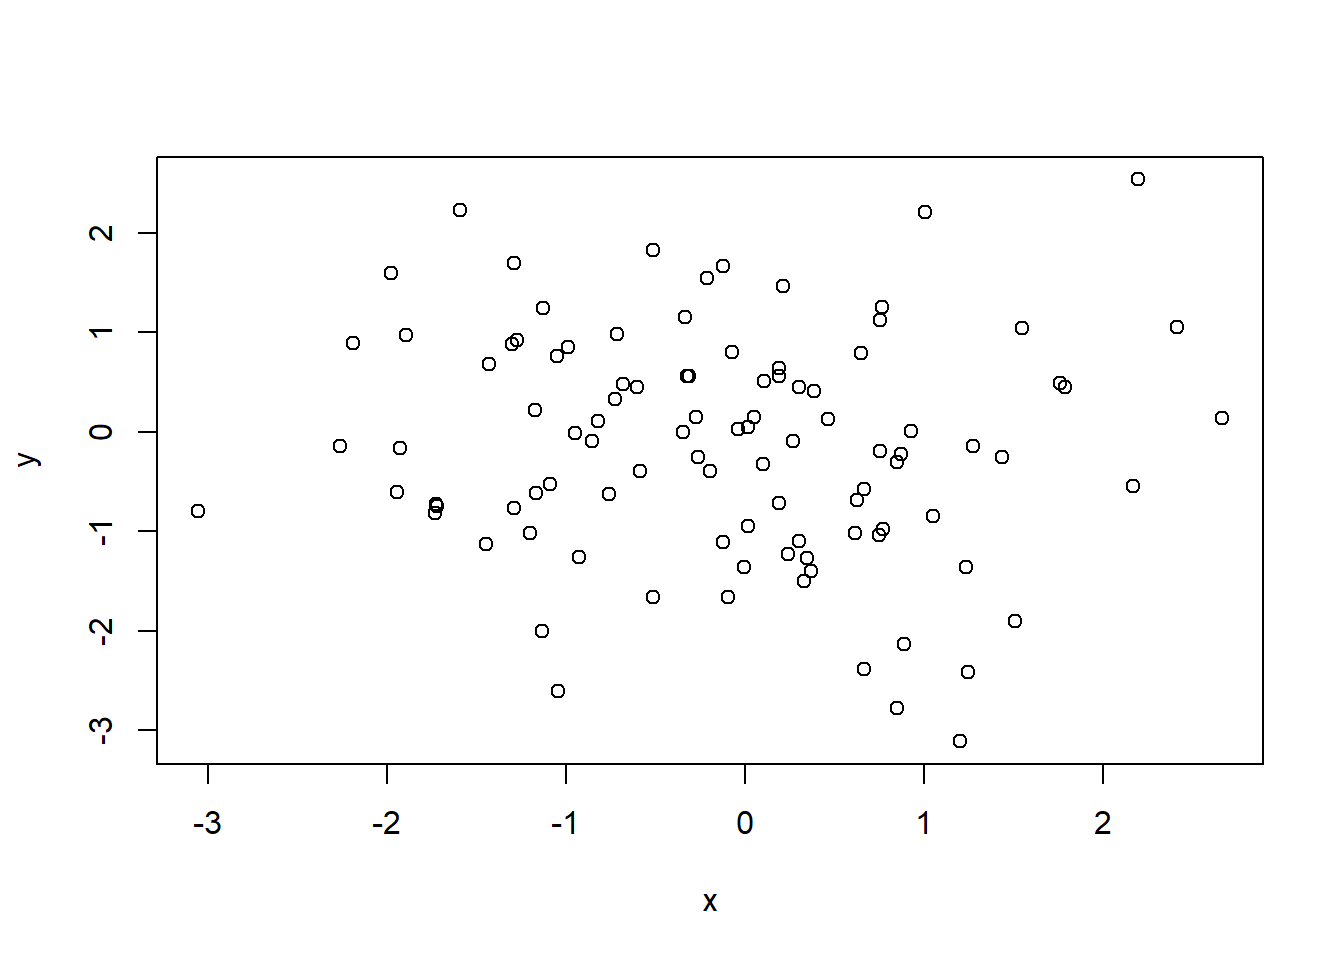
\includegraphics{test_files/figure-latex/unnamed-chunk-9-1} \caption{250个正例和500个负例情况下各种方法比较图}\label{fig:unnamed-chunk-9}
\end{figure}

\hypertarget{ux60c5ux51b53}{%
\subsubsection{情况3}\label{ux60c5ux51b53}}

接着本文将正例点和负例点控制在250和500个,将数据的维数提升到1000维,来比较各种方法的好坏。

\begin{longtable}[]{@{}cccccc@{}}
\caption{250个正例和500负例在1000维情况下各种方法指标比对}\tabularnewline
\toprule
method & Sensitivity & Specificity & FPR & FNR & ACC \\
\midrule
\endfirsthead
\toprule
method & Sensitivity & Specificity & FPR & FNR & ACC \\
\midrule
\endhead
awensvm & 67.24 & 91.30 & 8.69 & 32.75 & 82.00 \\
svm & 0.00 & 1.00 & 0.00 & 1.00 & 67.33 \\
logstic & 61.22 & 48.51 & 51.48 & 38.77 & 52.66 \\
BeSS & 92.45 & 1.00 & 0.00 & 7.54 & 97.33 \\
\bottomrule
\end{longtable}

可视化结果如下图所示。

\begin{figure}
\includegraphics{test_files/figure-latex/unnamed-chunk-11-1} \caption{250个正例和500个负例在1000维情况下各种方法比较图}\label{fig:unnamed-chunk-11}
\end{figure}

\hypertarget{ux603bux7ed3}{%
\subsubsection{总结}\label{ux603bux7ed3}}

通过在三种不同情况下对各种方法进行对比如下表所示。

\begin{table}[htbp]
  \centering
  \caption{各种方法在不同情况下各项指标对比}
    \resizebox{\linewidth}{!}{
    \begin{tabular}{|c|c|c|c|c|c|c|c|c|c|c|c|c|}
    \toprule
    方法    & \multicolumn{3}{c|}{awensvm} & \multicolumn{3}{c|}{SVM} & \multicolumn{3}{c|}{logstic} & \multicolumn{3}{c|}{BeSS} \\
    \midrule
    指标    & condition1 & condition2 & condition3 & condition1 & condition2 & condition3 & condition1 & condition2 & condition3 & condition1 & condition2 & condition3 \\
    \midrule
    Sensitivity & 73.46 & 69.49 & 67.24 & 80    & 12.5  & 0     & 66.07 & 89.58 & 61.22 & 90.19 & 100   & 92.45 \\
    \midrule
    Specificity & 73.46 & 93.4  & 91.3  & 57.14 & 100   & 1     & 73.43 & 76.47 & 48.51 & 88.4  & 100   & 1 \\
    \midrule
    FPR   & 18.3  & 6.59  & 8.69  & 2.8   & 0     & 0     & 29.68 & 23.52 & 51.48 & 7.2   & 0     & 0 \\
    \midrule
    FNR   & 18.57 & 30.5  & 32.75 & 4.76  & 42.6  & 1     & 28.78 & 10.41 & 38.77 & 7.57  & 0     & 7.54 \\
    \midrule
    ACC   & 77.5  & 84    & 82    & 60    & 72    & 67.33 & 70    & 78.28 & 52.66 & 89.16 & 100   & 97.33 \\
    \bottomrule
    \end{tabular}}%
  \label{tab:addlabel}%
\end{table}

通过对不同方法在三种情况下各个指标的对比,发现传统的分类方法如SVM和logstic方法,在比较正常的情况下还是有一定的效果。但是当类不平衡情况加重的情况下和维度扩张到\(p>>n\)的情况下时,传统的分类方法的各项指标会有显著的显著下降,造成了其无法正常的进行分类。而使用自适应加权弹性网支持向量机和\passthrough{\lstinline!BeSS!}方法可以克服这些情况,在不同情况下的各项指标显示,\passthrough{\lstinline!BeSS!}方法都显著优于\passthrough{\lstinline!AWENASVM!}方法。通过模拟计算,本文证明了\passthrough{\lstinline!BeSS!}方法在类不平衡和超高维情况下的优异表现。

\hypertarget{ux5bf9ux5b9eux8bc1ux6570ux636eux8fdbux884cux672aux52a0ux6743ux5efaux6a21}{%
\subsection{对实证数据进行未加权建模}\label{ux5bf9ux5b9eux8bc1ux6570ux636eux8fdbux884cux672aux52a0ux6743ux5efaux6a21}}

本文首先对该数据进行原始BeSS方法建模,具体参数及内容详见Wen\textsuperscript{{[}17{]}},本文中将回归模型设置为``binomial'',不进行权重加权时,每个样本默认的权重为1。建模的结果如图1所示。

\begin{figure}[h]  
\centering  
\includegraphics{pic1.eps}  
\caption{没有进行加权建模模型过程图}  
\label{建模过程图}  
\end{figure}

从图1可以看出,随着模型大小的增加,\(L(\beta)\)会出现一个降低的趋势,并且随着模型大小的变化,各个变量的系数也在图中有展示。该图横轴为模型规模即变量个数,上面第一幅图为损失函数的变化,下面表2为随着模型大小,各个特征系数。根据Zhu\textsuperscript{{[}11{]}}等人提出的SIC准则,在最终选择模型的时候并不只看损失函数的大小。

\begin{table}[htb]
\centering
\caption{ 建模过程中各项指标比较}
\begin{tabular}{ccccc}
\hline
Df  & Dev         & AIC         & BIC         & EBIC        \\ \hline
1   & 107.8423059 & 109.8423059 & 114.5281669 & 133.9361659 \\
120 & 0.000503217 & 240.0005032 & 802.3038169 & 3131.263695 \\
75  & 0.000234146 & 150.0002341 & 501.4398052 & 1957.039729 \\
47  & 0.00052864  & 94.00052864 & 314.2359932 & 1226.411945 \\
29  & 0.000561639 & 58.00056164 & 193.8905291 & 756.7224996 \\
18  & 0.000278811 & 36.00027881 & 120.3457759 & 469.6897575 \\
12  & 0.000197037 & 24.00019704 & 80.2305284  & 313.1265162 \\
8   & 0.000555819 & 16.00055582 & 53.4874434  & 208.7514352 \\
5   & 9.908629066 & 19.90862907 & 43.3379338  & 140.3779287 \\
7   & 0.008687521 & 14.00868752 & 46.80971415 & 182.665707  \\
6   & 0.008531852 & 12.00853185 & 40.12369753 & 156.5716914 \\ \hline
\end{tabular}
\end{table}

可以看出,随着模型规模即Df的变化,各项模型参数也随之变化,在各项指标之中,综合考虑,从而找到效果最好的模型。通过BeSS方法最终建模结果如下
\[
y=-1980.53+33.44*x_{1317}+45.08*x_{1750}+48.55*x_{1885}-48.88*x_{2318}+77.17*x_{4092}-3.11*x_{1317}
\]
脚标代表着筛选出的基因名称。因为是使用logstic回归模型,将阈值设定为0,输出混淆矩阵,通过混淆矩阵来评判该模型的好坏。

\begin{table}[htbp]
  \centering
  \caption{未进行加权建模的混淆矩阵}
    \begin{tabular}{|c|c|c|c|}
    \toprule
    \multicolumn{2}{|c|}{\multirow{4}[4]{*}{\textcolor[rgb]{ .2,  .2,  .2}{}}} & \multicolumn{2}{c|}{\multirow{3}[2]{*}{\textcolor[rgb]{ .2,  .2,  .2}{预测}}} \\
    \multicolumn{2}{|c|}{} & \multicolumn{2}{c|}{} \\
    \multicolumn{2}{|c|}{} & \multicolumn{2}{c|}{} \\
\cmidrule{3-4}    \multicolumn{2}{|c|}{} & \textcolor[rgb]{ .2,  .2,  .2}{-1} & \textcolor[rgb]{ .2,  .2,  .2}{1} \\
    \midrule
    \multicolumn{1}{|c|}{\multirow{4}[4]{*}{\textcolor[rgb]{ .2,  .2,  .2}{实际}}} & \multirow{2}[2]{*}{\textcolor[rgb]{ .2,  .2,  .2}{1}} & \multirow{2}[2]{*}{\textcolor[rgb]{ .2,  .2,  .2}{88}} & \multirow{2}[2]{*}{\textcolor[rgb]{ .2,  .2,  .2}{212}} \\
          &       &       &  \\
\cmidrule{2-4}          & \multirow{2}[2]{*}{\textcolor[rgb]{ .2,  .2,  .2}{-1}} & \multirow{2}[2]{*}{\textcolor[rgb]{ .2,  .2,  .2}{391}} & \multirow{2}[2]{*}{\textcolor[rgb]{ .2,  .2,  .2}{110}} \\
          &       &       &  \\
    \bottomrule
    \end{tabular}%
  \label{tab:addlabel}%
\end{table}

通过混淆矩阵看出,在没有使用加权方法进行建模时,混淆矩阵中实际为1的类被误分的比较多,其中\(N_{TP}=212,N_{FP}=88,N_{TN}=391,N_{FN}=110\),可以看出由于+1例较少,造成了比较严重的误分类情况,该情况下模型的ACC计算如下:\(P_{a c c}=\frac{N_{T P}+N_{T N}}{N_{T P}+N_{T N}+N_{F P}+N_{F N}}=0.75\)

\hypertarget{ux5bf9ux5b9eux8bc1ux6570ux636eux8fdbux884cux52a0ux6743ux5206ux7c7bux5efaux6a21}{%
\subsection{对实证数据进行加权分类建模}\label{ux5bf9ux5b9eux8bc1ux6570ux636eux8fdbux884cux52a0ux6743ux5206ux7c7bux5efaux6a21}}

通过之前提到的加权方法对输出进行加权之后建模。具体流程基本如上。使用加权处理之后,模型输出的模型选择图如图2所示。从图二看出,使用加权方法进行数据处理之后,数据的损失函数相比没有加权之前有了更大的降低,因此本文认为使用加权方法处理高维类不平衡的分类问题是有一定效果的。

\begin{figure}[h]  
\centering  
\includegraphics{pic2.eps}  
\caption{进行加权建模模型过程图}  
\label{建模过程图}  
\end{figure}

使用加权方法建立的最终模型如下所示: \[
y=-152.76-21.892*x_{2951}-26.25*x_{6611}+18.97*x_{6876}-12.21*x_{8349}+29.11*x_{8665}+7.36*x_{16245}
\]
通过使用加权的方法,筛选出的变量与没有加权的方法有了变化,这是因为每个样本的权重与没有加权的不一样了,这里的权重可以认为是数据的重要程度,在本文中,相当于是对较少的样本进行了加重处理,从而来针对类不平衡问题。接着看使用加权方法之后的混淆矩阵。使用加权处理之后,\(N_{TP}=242,N_{FP}=58,N_{TN}=429,N_{FN}=72\),这时的模型的\(P_{a c c}=0.83\)。通过对ACC值的比较发现,进行过加权处理的模型的ACC值提升了8个百分点,因此我们认为使用加权的方法能够对小样本下超高维数据类不平衡情况下提升分类准确率有一定的作用。

\begin{table}[htbp]
  \centering
  \caption{加权处理后的混淆矩阵}
    \begin{tabular}{|c|c|c|c|}
    \toprule
    \multicolumn{2}{|c|}{\multirow{4}[4]{*}{\textcolor[rgb]{ .2,  .2,  .2}{}}} & \multicolumn{2}{c|}{\multirow{3}[2]{*}{\textcolor[rgb]{ .2,  .2,  .2}{预测}}} \\
    \multicolumn{2}{|c|}{} & \multicolumn{2}{c|}{} \\
    \multicolumn{2}{|c|}{} & \multicolumn{2}{c|}{} \\
\cmidrule{3-4}    \multicolumn{2}{|c|}{} & \textcolor[rgb]{ .2,  .2,  .2}{-1} & \textcolor[rgb]{ .2,  .2,  .2}{1} \\
    \midrule
    \multicolumn{1}{|c|}{\multirow{4}[4]{*}{\textcolor[rgb]{ .2,  .2,  .2}{实际}}} & \multirow{2}[2]{*}{\textcolor[rgb]{ .2,  .2,  .2}{1}} & \multirow{2}[2]{*}{\textcolor[rgb]{ .2,  .2,  .2}{58}} & \multirow{2}[2]{*}{\textcolor[rgb]{ .2,  .2,  .2}{242}} \\
          &       &       &  \\
\cmidrule{2-4}          & \multirow{2}[2]{*}{\textcolor[rgb]{ .2,  .2,  .2}{-1}} & \multirow{2}[2]{*}{\textcolor[rgb]{ .2,  .2,  .2}{429}} & \multirow{2}[2]{*}{\textcolor[rgb]{ .2,  .2,  .2}{72}} \\
          &       &       &  \\
    \bottomrule
    \end{tabular}%
  \label{tab:addlabel}%
\end{table}

\hypertarget{ux603bux7ed3-1}{%
\section{总结}\label{ux603bux7ed3-1}}

本文通过将最新的最优子集法和数据驱动的自适应加权方法进行结合,讨论了该种方法的可行性,并在实际数据中通过模拟实验证明了该思想确实有一定的提升。但是由于种种原因限制,小样本和超高维数据不仅是有分类问题,也会有回归问题和聚类等问题,这些问题本文没有考虑到。结合现在实际情况,该种方法目前在医学诊断上面有不错的表现,但是本文认为,该种方法应该可以与目前比较火热的深度学习进行融合,如何在训练数据有限的情况下尽可能的建立最好的模型,来达到最好的效果,这个问题应该是比较有意义的。另外,关于最优子集算法这一问题,可以详细参考Fan\textsuperscript{{[}18{]}}等人的文章,在文章中详细证明了关于最优子集法的相关问题,能够对深刻理解最优子集算法有很好的提升。

最后,本文在撰写过程中不免会有许多疏漏和考虑不周的情况,还请各位读者指正。

\hypertarget{ux53c2ux8003ux6587ux732e}{%
\section*{参考文献}\label{ux53c2ux8003ux6587ux732e}}
\addcontentsline{toc}{section}{参考文献}

\hypertarget{refs}{}
\begin{CSLReferences}{0}{0}
\leavevmode\vadjust pre{\hypertarget{ref-LASSO1996}{}}%
\CSLLeftMargin{{[}1{]} }
\CSLRightInline{TIBSHIRANI R. {Regression Shrinkage and Selection Via
the Lasso}{[}J{]}. Journal of the Royal Statistical Society: Series B
(Methodological), 1996, 58(1): 267--288.}

\leavevmode\vadjust pre{\hypertarget{ref-SCAD2001}{}}%
\CSLLeftMargin{{[}2{]} }
\CSLRightInline{FAN J, LI R. {Variable selection via nonconcave
penalized likelihood and its oracle properties}{[}J{]}. Journal of the
American Statistical Association, 2001, 96(456): 1348--1360.}

\leavevmode\vadjust pre{\hypertarget{ref-Zou2005}{}}%
\CSLLeftMargin{{[}3{]} }
\CSLRightInline{ZOU H, HASTIE T. {Erratum: Regularization and variable
selection via the elastic net (Journal of the Royal Statistical Society.
Series B: Statistical Methodology (2005) 67 (301-320))}{[}J{]}. Journal
of the Royal Statistical Society. Series B: Statistical Methodology,
2005, 67(5): 768.}

\leavevmode\vadjust pre{\hypertarget{ref-leastangle2004}{}}%
\CSLLeftMargin{{[}4{]} }
\CSLRightInline{EFRON B, HASTIE T, JOHNSTONE I, 等. Least angle
regression{[}J{]}. Annals of Statistics, 2004, 32(2): 407--499.}

\leavevmode\vadjust pre{\hypertarget{ref-Meinshausen2006}{}}%
\CSLLeftMargin{{[}5{]} }
\CSLRightInline{MEINSHAUSEN N, BÜHLMANN P. {High-dimensional graphs and
variable selection with the Lasso}{[}J{]}. Annals of Statistics, 2006,
34(3): 1436--1462.}

\leavevmode\vadjust pre{\hypertarget{ref-Zou2006}{}}%
\CSLLeftMargin{{[}6{]} }
\CSLRightInline{ZOU H. {The adaptive lasso and its oracle
properties}{[}J{]}. Journal of the American Statistical Association,
2006, 101(476): 1418--1429.}

\leavevmode\vadjust pre{\hypertarget{ref-Candes2007}{}}%
\CSLLeftMargin{{[}7{]} }
\CSLRightInline{CANDES E, TAO T. {The Dantzig selector: Statistical
estimation when p is much larger than n}{[}J{]}. Annals of Statistics,
2007, 35(6): 2313--2351.}

\leavevmode\vadjust pre{\hypertarget{ref-Fan2008}{}}%
\CSLLeftMargin{{[}8{]} }
\CSLRightInline{FAN J, LV J. {Sure independence screening for ultrahigh
dimensional feature space}{[}J{]}. Journal of the Royal Statistical
Society. Series B: Statistical Methodology, 2008, 70(5): 849--911.}

\leavevmode\vadjust pre{\hypertarget{ref-Fan2010}{}}%
\CSLLeftMargin{{[}9{]} }
\CSLRightInline{FAN J, SONG R. {Sure independence screening in
generalized linear models with NP-dimensionality}{[}J{]}. Annals of
Statistics, 2010, 38(6): 3567--3604.}

\leavevmode\vadjust pre{\hypertarget{ref-Li2012}{}}%
\CSLLeftMargin{{[}10{]} }
\CSLRightInline{LI R, ZHONG W, ZHU L. {Feature screening via distance
correlation learning}{[}J{]}. Journal of the American Statistical
Association, 2012, 107(499): 1129--1139.}

\leavevmode\vadjust pre{\hypertarget{ref-Zhu2021}{}}%
\CSLLeftMargin{{[}11{]} }
\CSLRightInline{ZHU J, WEN C, ZHU J, 等. {A polynomial algorithm for
best-subset selection problem}{[}J{]}. Proceedings of the National
Academy of Sciences of the United States of America, 2021, 117(52):
33117--33123.}

\leavevmode\vadjust pre{\hypertarget{ref-hocking1967selection}{}}%
\CSLLeftMargin{{[}12{]} }
\CSLRightInline{HOCKING R R, LESLIE R. Selection of the best subset in
regression analysis{[}J{]}. Technometrics, Taylor \& Francis Group,
1967, 9(4): 531--540.}

\leavevmode\vadjust pre{\hypertarget{ref-li2008hybrid}{}}%
\CSLLeftMargin{{[}13{]} }
\CSLRightInline{LI P, QIAO P-L, LIU Y-C. A hybrid re-sampling method for
SVM learning from imbalanced data sets{[}C{]}//2008 Fifth International
Conference on Fuzzy Systems and Knowledge Discovery. IEEE, 2008, 2:
65--69.}

\leavevmode\vadjust pre{\hypertarget{ref-tang2008svms}{}}%
\CSLLeftMargin{{[}14{]} }
\CSLRightInline{TANG Y, ZHANG Y-Q, CHAWLA N V, 等. SVMs modeling for
highly imbalanced classification{[}J{]}. IEEE Transactions on Systems,
Man, and Cybernetics, Part B (Cybernetics), IEEE, 2008, 39(1):
281--288.}

\leavevmode\vadjust pre{\hypertarget{ref-zou2008svm}{}}%
\CSLLeftMargin{{[}15{]} }
\CSLRightInline{ZOU S, HUANG Y, WANG Y, 等. SVM learning from imbalanced
data by GA sampling for protein domain prediction{[}C{]}//2008 the 9th
international conference for young computer scientists. IEEE, 2008:
982--987.}

\leavevmode\vadjust pre{\hypertarget{ref-hwang2011new}{}}%
\CSLLeftMargin{{[}16{]} }
\CSLRightInline{HWANG J P, PARK S, KIM E. A new weighted approach to
imbalanced data classification problem via support vector machine with
quadratic cost function{[}J{]}. Expert Systems with Applications,
Elsevier, 2011, 38(7): 8580--8585.}

\leavevmode\vadjust pre{\hypertarget{ref-Wen2020}{}}%
\CSLLeftMargin{{[}17{]} }
\CSLRightInline{WEN C, ZHANG A, WANG X, 等. {Bess: An R package for best
subset selection in linear, logistic and cox proportional hazards
models}{[}J{]}. Journal of Statistical Software, 2020, 94(4): 1--24.}

\leavevmode\vadjust pre{\hypertarget{ref-Fan2020a}{}}%
\CSLLeftMargin{{[}18{]} }
\CSLRightInline{FAN J, ZHU Z. {When is best subset selection the
{《best》}?}{[}J{]}. arXiv, 2020.}

\end{CSLReferences}

\end{document}
